
Cando se prende un ordenador cárgase parte do kernel do  sistema operativo en memoria. Espértase ó ordenador para que recoñeza á CPU, a memoria, as unidades de disco e calquera outro dispositivo conectado sexa o teclado, o rato ou a impresora. Verifícase que no existan erros de conexión e que todos os dispositivos estean preparados para traballar axeitadamente. A este primeiro diagnóstico chámaselle POST.\\

Tras o arranque do ordenador o sistema operativo cárgase en memoria e permanece alí. O usuario xa pode interacionar con el para acceder ós recursos da máquina grazas a que actúa en segundo plano. Só deixa de executarse cando se apaga a máquina. 

Actuando en segundo plano o sistema operativo mantén unhas táboas que lle permiten saber os recursos que están libres.  A asignación de recursos realízase segundo a dispoñibilidade dos mesmos e a prioridade dos programas, debéndose resolver os conflitos que aparecen polas peticións simultáneas. Especial mención reviste a recuperación dos recursos cando os programas xa non os precisan. Unha mala recuperación de recursos pode facer que o SO considere que xa non lle queda memoria dispoñible cando, en realidade, si a ten.

Os servizos que ofrece o sistema operativo adóitanse agrupar segundo a súa funcionalidade en varios compoñentes a través dunha interface de chamadas ao sistema. Os programas poderán elixir sobre que servizo queren executar, pero non poderán misturar varios servizos á vez. Na figura \ref{servizos} podemos ver un esquema dos servizos que ofrece o sistema operativo.\\

\begin{figure} 
\begin{center}
\caption{Esquema das funcións dun sistema operativo}
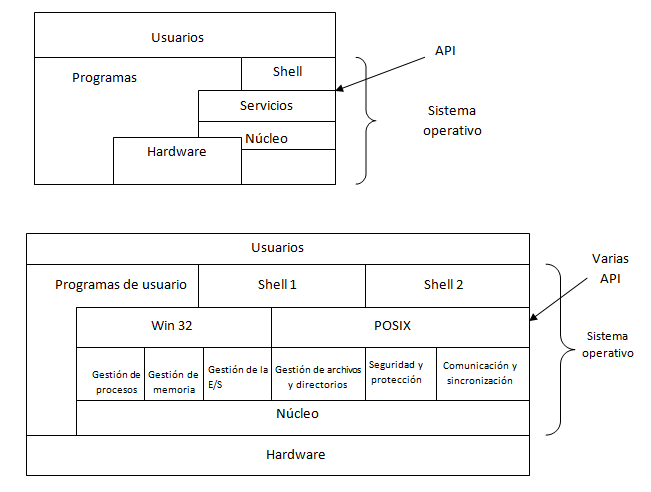
\includegraphics[width=0.9\textwidth]{./debuxos/unid.png}
\label{servizos}
\end{center}
\end{figure}
